\documentclass{article}


\usepackage[margin=1in]{geometry}
\usepackage{mathtools} %also loads amsmath
\usepackage{amssymb, bbm}

\usepackage[backend=biber,
	style=alphabetic,
	%	citestyle=authoryear,
	natbib=true,
	url=true, 
	doi=true]{biblatex}

%\usepackage{blkarray} % for matrices with labels
\usepackage{microtype}
\usepackage{relsize}
\usepackage{environ}% http://ctan.org/pkg/environ; for capturing body as a parameter for idxmats
\usepackage{tikz}
	\usetikzlibrary{positioning,fit,calc, decorations, arrows, shapes, shapes.geometric}
	\usetikzlibrary{cd}
	
	\pgfdeclaredecoration{arrows}{draw}{
		\state{draw}[width=\pgfdecoratedinputsegmentlength]{%
			\path [every arrow subpath/.try] \pgfextra{%
				\pgfpathmoveto{\pgfpointdecoratedinputsegmentfirst}%
				\pgfpathlineto{\pgfpointdecoratedinputsegmentlast}%
			};
	}}
	%%%%%%%%%%%%
	\tikzset{center base/.style={baseline={([yshift=-.8ex]current bounding box.center)}}}
	
	\tikzset{dpadded/.style={rounded corners=2, inner sep=0.9em, draw, outer sep=0.4em, fill=gray, fill opacity=0.08, text opacity=1}}
	\tikzset{active/.style={fill=blue, fill opacity=0.1}}
	\tikzset{square/.style={regular polygon,regular polygon sides=4, rounded corners = 0}}
	\tikzset{octagon/.style={regular polygon,regular polygon sides=8, rounded corners = 0}}
	
	
	\tikzset{alternative/.style args={#1|#2|#3}{name=#1, circle, fill, inner sep=1pt,label={[name={lab-#1},gray!30!black]#3:\scriptsize #2}} }
	
	
	\tikzset{bpt/.style args={#1|#2}{alternative={#1|#2|above}} }
	\tikzset{tpt/.style args={#1|#2}{alternative={#1|#2|below}} }
	\tikzset{lpt/.style args={#1|#2}{alternative={#1|#2|left}} }
	\tikzset{rpt/.style args={#1|#2}{alternative={#1|#2|right}} }
	\tikzset{pt/.style args={#1}{alternative={#1|#1|above}} }
	

	\tikzset{mpt/.style args={#1|#2}{name=#1, circle, fill, inner sep=1pt,label={[name={lab-#1},gray]\scriptsize #2}} }
	\tikzset{pt/.style args={#1}{name=#1, circle, fill, inner sep=1pt,label={[name={lab-#1},gray]\scriptsize #1}} }
	
		
		 %\foreach \x in {#1}{(\x) (lab-\x) } 
		 
	\tikzset{Dom/.style args={#1 (#2) around #3}{dpadded, name=#2, label={[name={lab-#2},align=center] #1}, fit={ #3 } }}
	\tikzset{bDom/.style args={#1 (#2) around #3}{dpadded, name=#2, label={[name={lab-#2},align=center]below:#1}, fit={ #3 } }}
	\tikzset{arr/.style={draw, ->, thick, shorten <=3pt, shorten >=3pt}}
	\tikzset{archain/.style args={#1}{arr, every arrow subpath/.style={draw,arr, #1}, decoration=arrows, decorate}}
	%\tikzset{every label/.append style={text=red, font=\scriptsize}}
	\tikzset{dpad/.style args={#1}{every matrix/.append style={nodes={dpadded, #1}}}}
	\tikzset{light pad/.style={outer sep=0.2em, inner sep=0.5em, draw=gray!50}}
	
	
	\newcommand\cmergearr[4]{
		\draw[arr,-] (#1) -- (#4) -- (#2);
		\draw[arr, shorten <=0] (#4) -- (#3);
	}
	\newcommand\mergearr[3]{
		\coordinate (center-#1#2#3) at (barycentric cs:#1=1,#2=1,#3=1.2);
		\cmergearr{#1}{#2}{#3}{center-#1#2#3}
	}

\NewEnviron{ctikzpicture}{\begin{center}\expandafter\begin{tikzpicture}\BODY\end{tikzpicture}\end{center}}
%\newenvironment{ctikzpicture}
%	{\begin{center}\begin{tikzpicture}}
%	{\end{tikzpicture}\end{center}}

\usepackage{color}
\definecolor{deepgreen}{rgb}{0,0.5,0}

\usepackage[colorlinks=true, citecolor=deepgreen]{hyperref}


\setlength{\skip\footins}{1cm}
\setlength{\footnotesep}{0.4cm}


\usepackage{stmaryrd}
\usepackage{trimclip}

\makeatletter
\DeclareRobustCommand{\shortto}{%
	\mathrel{\mathpalette\short@to\relax}%
}

\newcommand{\short@to}[2]{%
	\mkern2mu
	\clipbox{{.5\width} 0 0 0}{$\m@th#1\vphantom{+}{\shortrightarrow}$}%
}
\makeatother

\usepackage{parskip}
\usepackage{amsthm, thmtools}
\usepackage{
	nameref,%\nameref
	hyperref,%\autoref
	% n.b. \Autoref is defined by thmtools
	cleveref,% \cref
	% n.b. cleveref after! hyperref
}

\hypersetup{colorlinks=true, linkcolor=blue, urlcolor=magenta}

\begingroup
\makeatletter
\@for\theoremstyle:=definition,remark,plain\do{%
	\expandafter\g@addto@macro\csname th@\theoremstyle\endcsname{%
		\addtolength\thm@preskip\parskip
	}%
}
\endgroup
\makeatother

\theoremstyle{plain}
\newtheorem{theorem}{Theorem}[section]
\newtheorem{coro}{Corollary}[theorem]
\newtheorem{prop}[theorem]{Proposition}
\newtheorem{lemma}[theorem]{Lemma}
\newtheorem{fact}[theorem]{Fact}
\newtheorem{conj}[theorem]{Conjecture}

\theoremstyle{definition}
\newtheorem{defn}{Definition}[section]
\newtheorem*{defn*}{Definition}
\newtheorem{examplex}{Example}[section]
\newenvironment{example}
	{\pushQED{\qed}\renewcommand{\qedsymbol}{$\triangle$}\examplex}
	{\popQED\endexamplex\vspace{-1em}\rule{1cm}{0.7pt}\vspace{0.5em}}

\theoremstyle{remark}
\newtheorem*{remark}{Remark}

\usepackage{xstring}
\usepackage{enumitem}

\DeclarePairedDelimiterX{\infdivx}[2]{(}{)}{%
	#1\;\delimsize\|\;#2%
}
\newcommand{\kldiv}{D_\mathrm{KL}\infdivx}
%\DeclarePairedDelimiter{\norm}{\lVert}{\rVert}

%\newcommand\duplicat[1]{\gdef\mylist{}\foreach \x in {#1}{\xdef\mylist{\mylist (\x) (lab-\x) }}\mylist} %% this doesn't work :((
\newcommand\lab[1]{(#1)(lab-#1)}


\newcommand{\CI}{\mathrel{\perp\mspace{-10mu}\perp}}
\newcommand\E{{\mathbb E}}


\newcommand{\todo}[1]{{\color{red}\large\textbf{[}{\normalsize\texttt{todo:} \itshape#1}\textbf{]}}}
\newcommand{\note}[1]{{\color{blue}\large\textbf{[}{\normalsize\texttt{note:} \itshape#1}\textbf{]}}}

\newcommand\geqc{\succcurlyeq}
\newcommand\leqc{\preccurlyeq}
\newcommand\mat[1]{\mathbf #1}
\newcommand{\indi}[1]{\mathbbm{1}_{\left[\vphantom{\big[}#1 \vphantom{\big]}\right]}}
\newcommand\m[1]{\mathbf m_{\mathsf #1}}
\def\cpm#1(#2|#3){\mathbf #1 \left[ #2 \middle|#3\right]}


\newcommand\recall[1]{\expandarg\cref{#1}:\vspace{-1em} \begingroup\small\color{gray!80!black}\begin{quotation} \expandafter\csname #1\endcsname* \end{quotation}\endgroup }

%OMG THIS WORKS

\def\wrapwith#1[#2;#3]{
	\expandafter#2{\expandarg\StrBefore{#1}{,}}
	\expandarg\StrBehind{#1}{,}[\tmp] 
	\xdef\tmp{\expandafter\unexpanded\expandafter{\tmp}}
	#3
	\expandarg\IfSubStr{\tmp}{,}{\wrapwith{\tmp}[#2;{#3}]}{ \expandafter#2{\tmp} }
}
\def\hwrapcells#1[#2]{\wrapwith#1[#2;&]}
\def\vwrapcells#1[#2]{\wrapwith#1[#2;\\]}



\newsavebox{\idxmatsavebox}
\def\makeinvisibleidxstyle#1#2{\phantom{\hbox{#1#2}}}
\newenvironment{idxmatphant}[4][\footnotesize\color{gray}\text]{%
	\def\idxstyle{#1}
	\def\colitems{#3}
	\def\rowitems{#2}
	\def\phantitems{#4}
	\begin{lrbox}{\idxmatsavebox}$
	\begin{matrix}  \begin{matrix} \hwrapcells{\colitems}[\idxstyle]  \end{matrix} \\[0.1em]
		\left[ 
		\begin{matrix}
			\hwrapcells{\phantitems}[\expandafter\makeinvisibleidxstyle\idxstyle]  \\[-1em]
	}{
		\end{matrix}\right]		&\hspace{-0.5em}\begin{matrix*}[l] \vwrapcells{\rowitems}[\idxstyle] \end{matrix*}
	\end{matrix}
	$\end{lrbox}
	\raisebox{0.75em}{\usebox\idxmatsavebox}
%	\vspace{-0.5em}
}

\newenvironment{idxmat}[3][\footnotesize\color{gray}\text]
	{\begingroup\idxmatphant[#1]{#2}{#3}{#3}}
	{\endidxmatphant\endgroup}

\newenvironment{sqidxmat}[2][\footnotesize\color{gray}\text]
	{\begingroup\idxmat[#1]{#2}{#2}}
	{\endidxmat\endgroup}
	
	
%%%%%%%%%%%%
% better alignment for cases
\makeatletter
\renewenvironment{cases}[1][l]{\matrix@check\cases\env@cases{#1}}{\endarray\right.}
\def\env@cases#1{%
	\let\@ifnextchar\new@ifnextchar
	\left\lbrace\def\arraystretch{1.2}%
	\array{@{}#1@{\quad}l@{}}}
\makeatother

\usepackage{subcaption}
\usepackage{comment}
%\includecomment{vfull}
%\includecomment{vcat}
\excludecomment{vfull}
\excludecomment{vcat}
%\excludecomment{nonintro}


%%%%%% Commands to highlihght changes in the document.
\definecolor{note-fg}{rgb}{0.0,.4,0.2}
%\newcommand\changed[1]{\colorbox{light gray}{\parbox{\linewidth}{#1}}}
\newcommand\changed[1]{{\color{note-fg} #1}}
\newcommand\changeon{\color{note-fg} }
\newcommand\changeoff{\color{black} }

\usetikzlibrary{external}
\tikzexternalize[prefix=tikz/]  % activate!

\AtBeginEnvironment{tikzcd}{\tikzexternaldisable} %... except careful of tikzcd...
\AtEndEnvironment{tikzcd}{\tikzexternalenable}



\usepackage[nointegrals]{ wasysym }

\addbibresource{../refs.bib}
\addbibresource{../uncertainty.bib}
\addbibresource{../maths.bib}


% symbols for genders, hour glass.
\newcommand{\mfem}{\mathclap\female\male}
\newsavebox{\hourglassbox}
\savebox{\hourglassbox}{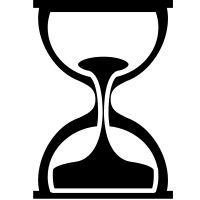
\includegraphics[height=.8em]{hourglass.png}}
\newcommand\hourglass{\usebox{\hourglassbox}}

%%% What do I even call them anyway?
\newcommand{\modelname}{Probabilistic Dependency Graph}
\newcommand{\modelnames}{Probabilistic Dependency Graphs}
\newcommand{\MN}{PDG}
\newcommand{\MNs}{PDGs}

%%%%%%%%%%%%%%%% SHORTCUTS FOR COMMONLY USED THINGS %%%%%%%%%%

\newcommand\Set{\textbf{Set}}
\newcommand\FinSet{\textbf{FinSet}}
\newcommand\MeasSet{\textbf{MeasSet}}
\newcommand\MaxEnt{{\substack{\mathbf{Max}\\\mathbf{Ent}}}}
%\def\bmu[#1|#2]{\boldsymbol\mu\boldsymbol{[} #1 \boldsymbol{|} #2 \boldsymbol{]}}
\newcommand\bmu{\boldsymbol{\mu}}

\title{Dependency Graphs}
\author{Oliver Richardson,  \texttt{oli@cs.cornell.edu}}

\begin{document}
	\maketitle

	\begin{abstract}
		Graphical models have enjoyed substantial success in compressing probability distributions over joint settings of random variables, by encoding correlations locally in links, and making use of independence assumptions elsewhere. Still, due to the fact that they are committed to representing a single consistent distribution, they are not expressive enough to represent common mental states of agents who may not have a perfectly logical coherent . Unrelatedly, the process of modifying graphical models by adding or removing nodes/links can be quite expensive and changes the underlying space, making it more difficult to make use of the intuitive modularity that they seem to offer.
		
		We introduce \modelnames (\MNs) to combat these issues. \MNs\ are like unshackled Bayesian nets, interpreted more locally and whose links are interpreted as conditional sub-distributions. The result is a “graphical model” in a looser sense which may not always be either complete or consistent (from the perspective of a distribution), which can be easily combined with graph operations. We find that by solely altering the set of nodes and links and then running consistency reduction algorithm (one of which is a generalized version of belief propagation), we can recover important capabilities of Bayesian networks, such as the ability to estimate conditional and marginal distributions given observations, belief updating via Jeffrey’s rule. Further afield, we discover that this process also naturally models simple learning algorithms, and acting according to a decision rule (see the other paper for more). Bayesian networks, and to some extent, factor graphs, can be seen as special cases of \MNs.
	\end{abstract}

	\tableofcontents

	\section{Introduction}



	%JOE-OUTLINE-1
		% Although inconsistency was our major motivation, I’m not sure that that’s how I would write  the introduction.  Here’s a possible alternative:
		% There are a number of quite successful graphical representations of uncertainty.  We’re going to introduce one more.  What makes our novel and interesting?  Two things:  (1) it can represent local information and (2) it can represent inconsistency.  Here are some examples to show that both features are quite useful 
		%in practice.  The examples will also give some intuition for our representation.  [[GIVE EXAMPLES.]]  Point out that our approach seems cognitively
		%simpler.  Discuss (at a high level) the two possible semantics for the language.  Say that the “weighted probabilities” approach has two significant advantages over the more obvious “set of probability measures”  approach:  (1) It allows us to consider inconsistent scenarios, since the distributions do not have to be consistent with the graph.  (2) It gives us a natural way of going from a local picture to a global one; there are various choices, and we can consider the “best” one(s).  (3) It allows us to connect our approach to Bayesian networks (and factor graphs?) in a straightforward way.    
		
	%JOE-OUTLINE-2
%		Our initial motivation was to
%		model preference change, which we felt was in part driven by
%		inconsistencies.  But standard graphical model representations don't
%		allow us to model inconsistency.  We were particularly interested in
%		being able to model "local" inconsistency.  That is, most of your
%		information is correct; there's just a small part that's inconsistent.
%		As we shall see, the ability to model such locality turns out to be
%		useful even in a setting where an agent's beliefs are consistent.
	
	{\color{blue}
%	\textbf{Outline, from your suggested one.}
%	There are many representations of uncertainty. Probability is one of them. Graphical models are a compact representations of spaces and distributions on them. 
%	The most important feature is not the fact that the model takes the form of a graph, nor that the variables are intelligible, but rather
%		that both (1) the space of possible worlds, and (2) the distribution over them are both determined implicitly and compactly.
%	However, these representations are ultimately committed to representing probability distributions; I argue that the graphical model bit is a
	}

	
	
	\changed{Storing your beliefs in the form of a single probability distribution over a fixed set of possibilities is hard work. Before having any experience,} you must first conceptualize the set of all worlds you could ever consider possible. 
	Then, each time you acquire knowledge, you need to know exactly how much you trust it, and do substantial book-keeping just to maintain a valid mental state in the form of a prior over these possible worlds.
	%
	\changed{One primary reason this feels like a handicap is due to the} \textit{lack of modularity}: there is no way to conceptualize new worlds, and it is only possible to combine observations with an existing prior (that you trust). \changed{As a result, anything you might do that doesn't necessarily identify a distribution---such as combining partial observations, looking at only part of your knowledge, adopting beliefs without considering their impact on all possible worlds, or simply forgetting your prior---leaves you in a rough spot because the resulting mental state cannot be represented}.
	%	
	Why tie yourself down this way? The big payoff is \textit{guaranteed consistency}. Having inconsistent beliefs leads to arbitrarily bad conclusions, and leave you vulnerable to unbounded pain in the form of dutch book arguments; the engineering ethos suggests it is best to avoid such things by design.
	
	
	Abiding by these restrictions seems empirically too difficult for humans, \changed{but there is still nonetheless a strong case that we should} approximate it as best we can, especially given the freedom to construct arbitrary artificial agents. Fortunately, there are many tools to make the problem tractable; of particular relevance are graphical models, which offer a compact, implicit representation of possible worlds as settings of random variables, and of a distribution over them in terms of local information. Graphical models even offer modularity (to various extents), but the existing ones are still beholden to the restrictions above: updating is still restrictive and expensive, and consistency is enforced by the representation, in a way which cripples promises of modularity.\footnote{This avoidance of inconsistency is actually the reason that adding arbitrary nodes to graphical models is problematic: to add a node to a network, it has to satisfy the appropriate independence properties, lest the network actually represent two distinct beliefs about one thing. Of course, knowing this for certain is a very strong assumption, and hence you cannot safely add nodes to graphical models without already knowing a lot about the variable---which begs the question: if your mental state is only what's in the graphical model, how did you get this knowledge of a new variable?}
	
	While we share the distaste for inconsistency, awareness of it can be a useful resource for seeking truth, and knowledge that there isn't even though there could have been, is a valuable safeguard. Worse than merely missing this opportunity, disallowing inconsistency by construction can sweep problems under the rug (see \cref{sec:consistency-ethos} for the full argument). In light of this, we introduce a more general representation of knowledge and uncertainty in the form of a graphical model capable of representing inconsistent belief states, which we call \modelnames\ (\MNs). Special cases of \MNs\ include Bayesian Networks and they can also mostly emulate (but are better behaved than) factor graphs. The extra flexibility makes them easier to use, and surprisingly, they enjoy additional properties which make them more useful than some specific variants, which we list in \cref{sec:list-of-benefits}.
%	Why use a graphical model at all?
%	\begin{enumerate}[nosep]
%		\item Compressed, implicit representation of a giant joint distribution, making use of independence
%		\item An intuitive way of communicating complex models.
%		\item A more local knowledge representation
%	\end{enumerate}
	To get a feel for what \MNs\ are and how they differ from other graphical models, it is helpful to see examples.
	

	%%%%%%%%%%%%%%%%%%%


	\begin{example} \label{ex:planet}
		Suppose we have a belief about how size and composition affect the habitability of a planet: say we're astrobiologists, and we have some sense of how likely we are to find life on a given planet, supposing we knew its size (big or small) and its composition (mostly made of rocks vs gas). That is to say, we have a conditional probability table:
		
		\begin{center}
			$\Pr(\text{Life} ~|~ \text{Size}, \text{Comp}) = 
			\begin{idxmat}{{big, rocky}, {small,rocky}, {big, gasseous}, {small,gasseous}}{life, no life}
				.1 & .9 \\
				.2 & .8 \\
				.05 & 0.95 \\
				0.00001 & 0.99999
			\end{idxmat} 
			\qquad$
			\begin{tikzpicture}[center base]
			\node[dpadded,light pad,fill opacity=0] (SS) at (-0.4, 1.2) {Size};
			\node[dpadded,light pad,fill opacity=0] (CC) at (3.4, 1.2) {Composition};
			\node[dpadded,light pad,fill opacity=0] (LL) at (1.2,0) {Life};
			\draw[arr] (CC) -- (LL);
			\draw[arr] (SS) -- (LL);
			\end{tikzpicture}		
		\end{center}
		\vspace{1em}
	
		This one conditional probability table cannot constitute a full Bayesian network. It is indeed a fragment of the Bayesian Network on the right, but in order to interpret the picture as a BN, we would \changed{also generally insist that there were also distributions over the values of  the root nodes} `Size' and `Composition'---things we may not know anything about.\footnote{Models like these are well known to hardcore probabilists as well. In statistical learning theory, an `incomplete' model like this is a discriminative (or conditional) model, as compared to a generative one.}
		While such a mental state is under-constrained from the perspective of probability, it is certainly falsifiable and \emph{seems like knowledge}. This is perhaps the most common challenge to the idea that belief states are probability distributions, and by extension to the universality of the Bayesian Networks which represent them.

		\changed{The opposite problem, though less appreciated, also occurs: just as it is impossible to represent an under-constrained distribution with a Bayesian Network, so too is it impossible to represent an over-constrained one. Patching this requires the more radical fix we present in the form of a \MN.} Suppose our biologist friend now reminds us that life requires water, and gives us a probability estimate for the existence of life on a planet, with and without water. We trust this friend completely, and totally believe these probabilities. Unfortunately, but there's no way to place it as the parent of the $L$ node, because we don't know what the correlations are between water, size, and composition; neither are we prepared to give a probability of live given a full description of the three, and may not even have the space to keep such a thing.\footnote{If \textit{Size} and \textit{Composition} each had $\approx\sqrt{N}$ elements, and \textit{Water} had $\approx N$ elements, it would be $O(N^2)$ to store a full joint table, compared to $O(N)$ for the two individual ones.} %At this point the Bayesian Network is not at all a convenient way of storing the information at hand.
		Let $S, C, W, L$ be shortenings of Size, Composition, Water, and Life, respectively.
		Intuitively, we want to draw instead a picture that looks more like this:

		\begin{center}
		\begin{tikzpicture}
			\node[dpadded] (S) at (-0.4, 2) {$S$};
			\node[dpadded] (C) at (3, 2) {$C$};
			\node[dpadded] (L) at (1.3,0) {$L$};
			\node[dpadded] (W) at (-2,0) {$W$};
			\cmergearr{S}{C}{L}{1.3,1.1}
			\draw[arr] (W) -- (L);
		\end{tikzpicture}
		\end{center}
	
		which represents having two conditional probability tables on $L$: one from $S \times C$ and the other from $W$. This would allow us to combine the two facts that we know, without also providing much more information than we're prepared to equivocate on. It is worth noting that there is now a possibility of being inconsistent, in the sense that is possible to specify the conditional distributions in the links in such a way that no joint distribution on all variables will marginalize out to them --- for instance, if all estimates of $L$ from the $W$ are strictly smaller than any probability estimate of $L$ from $S \times C$.
	\end{example}

	\begin{example}\label{ex:smoking}
		Consider the classic example used to introduce Bayesian nets, in which the four variables are interest are booleans indicating whether a person ($C$) develops cancer, ($S$) smokes, ($SH$) is exposed to 2nd hand smoke, and ($PS$) has parents who smoke, presented graphically in \cref{fig:smoking-bn+pdg}.
		\begin{figure}[h!]
			\centering
			
			\begin{subfigure}[b]{0.3\textwidth}
				\begin{tikzcd}[center base, column sep=1.8em, row sep=1.3em, dpad={fill opacity=0, draw=gray}]
				& S \ar[dr] \\
				PS \ar[ur]\ar[dr] && C \\
				& SH \ar[ur]
				\end{tikzcd}
			\caption{Bayesian Network}
			\end{subfigure}
			\hspace{2em}\vline\hspace{2em}
			\begin{subfigure}[b]{0.5\textwidth}
				\begin{tikzpicture}[center base]
				\node[dpadded] (1) at (0,0) {true};
				\node[dpadded] (PS) at (2,0) {$PS$};
				\node[dpadded] (S) at (4, 1.4) {$S$};
				\node[dpadded] (SH) at (4, -1.4) {$SH$};
				\node[dpadded] (C) at (6.5,0) {$C$};
				
				\draw[arr] (1) -- (PS);
				\draw[arr] (PS) -- (S);
				\draw[arr] (PS) -- (SH);
				\cmergearr{SH}{S}{C}{5.1,0}
				\end{tikzpicture}
				\caption{Corresponding \MN}
			\end{subfigure}
		
			\caption{Both graphical models representing the conditional relationships in \cref{ex:smoking}}
			\label{fig:smoking-bn+pdg}
		\end{figure}
		
		This is a compact representation of a joint distribution over all four variables, which achieves compactness by taking advantage of independence between variables. It encodes an assumption that every node is independent of its non-descendants given its parents.
		
		Most of the time, we do not make the independence assumption because we know for certain that the variables are independent; rather, we just suspect that the identified links are by much more important than the others. Determining for sure that smoking  and second hand smoke are independent, controlling for parents' smoking habits, would extremely difficult, and to do properly would require much more empiricism to validate. \changed{So why make such assumptions? Because} BNs are designed to be a compact implicit description of a probability distribution. 
		
		


		The node on the far left is a special node which only takes one value, and allows us to represent unconditional distributions as arrows, visually making clear the difference between a lack of distribution, and an unconditional one. 
		
		Now, suppose you read a very thorough empirical study which demonstrates that people who use tanning beds have a 10\% incidence of cancer, compared with 1\% in the control. Just as in the previous example, this cannot be encoded directly into the Bayesian Network. 
		The \MN\, on the other hand, has no trouble, and is simply the union of the two pieces of information:
		
		\begin{center}
			\begin{tikzpicture}
			\node[dpadded] (1) at (0,0) {true};
			\node[dpadded] (PS) at (2,0) {$PS$};
			\node[dpadded, fill opacity=0.16] (S) at (4, 1.4) {$S$};
			\node[dpadded, fill opacity=0.16] (SH) at (4, -1.4) {$SH$};
			\node[dpadded, fill opacity=0.16] (C) at (6.5,0) {$C$};
			\node[dpadded, fill opacity=0.16] (T) at (8.5,0) {$T$};
			
			\draw[arr] (1) -- (PS);
			\draw[arr] (PS) -- (S);
			\draw[arr] (PS) -- (SH);
			\cmergearr{SH}{S}{C}{5.1,0}
			\draw[arr] (T) -- (C);
			\end{tikzpicture}
		\end{center}
		Note that the right half of the diagram (shaded slightly darker) has the same topology as in example \ref{ex:planet}.
	\end{example}


	\subsection{Factor Graphs}
	
	\begin{example}[continues=ex:planet]
		The probabilists in us might not be willing to so easily give up the notion that this data ought to define a probability distribution, at least implicitly. 
		% We presumably already have a prior over everything, and in the event that we d
		%Bayesian networks are insufficient to represent this epistemic state is because the state is not a distribution and hence invalid? 
		Maybe there's something simple we can do to turn it into one? It turns out that we can (almost always) \changed{simultaneously get a distribution and commit to preserving the relative ratios of the specified probabilities within the links, while also more clearly exposing our independence assumptions. 		
		%specified to be probability distribution. If we had had a prior, perhaps we could have ``conditioned'' it on the new probability information that our colleague gave us.%
		%\footnote{
		%	``Conditioned'' gets quotation marks because the statement is not an event --- it is not information about the actual world $(S,C,L,W)$, but a meta-statement about probabilities. A probabilist can now avoid this by incorporating the things that a colleague can say into their mental model, and conditioning on the things that are said, which are now truly events. There are two issues with this. First, thsi runs into the problem that you already needed to have all worlds modeled in your head. Even if you allow yourself to form new concepts and worlds as the come to attention,  
		%	}
		 %	Together with the perspective that a Bayesian Network really encodes independence, this line of thought might cause one to think that the problem was a restrictive class of graphical model. Perhaps really we wanted a factor graph:
		This can be done by} treating the conditional distributions $p(L =l \mid S=s, C=c)$ and $p(L=l \mid W=w)$ as \emph{factors}, which multiplied together give the relative probability density of any setting of variables $S \times C \times W \times L$
		\[ \Pr(s, c, w, l) \propto \phi_1(s,c,l) \phi_2(w,l) \]
		where $\phi_1(s,c,l) = p(L=l \mid S=s, C=c)$, $\phi_2(w,l) = p(L=l\mid W=w)$. This can also be represented graphically, with a \emph{factor graph}---a commonly used graphical model hailed as a strict generalization of Bayesian Networks and Markov networks.
		
		\begin{center}
		\begin{tikzpicture}
			\node[dpadded,inner sep=0.6em, circle] (S) at (-0.4, 2) {$S$};
			\node[dpadded,inner sep=0.6em, circle] (C) at (3, 2) {$C$};
			\node[dpadded,inner sep=0.6em, circle] (L) at (1.3,0) {$L$};
			\node[dpadded,inner sep=0.6em, circle] (W) at (-2,0) {$W$};
			
			\node[light pad] (f1) at (1.3, 1.3){$\phi_1$};
			\node[light pad] (f2) at (-0.3, 0){$\phi_2$};
						
			\draw[thick] (S) -- (f1) -- (C) (f1) -- (L);
			\draw[thick] (W) -- (f2) -- (L);
		\end{tikzpicture}
		\end{center}
	 	\changed{In this diagram, circles represent variables, and the boxes represent factors that depend on variables they connect to.}
		This is a lot more modular (we can add and remove factors as we like). We now have a distribution that combines our beliefs, but this is not really what we were thinking of earlier. Beyond simply the inevitable effects \changed{of representing our knowledge as a distribution, such as forcing us to implicitly adopt marginal distributions over the variables $S,C$, and $W$, a product of factors has additional undesirable properties that are not shared by \MNs:}

		\begin{enumerate}
			\item We can't weight the pieces of information differently. Though the scale of each factor $\phi_i$ gives us a degree of freedom in which to encode this information, it cannot be used, as $(a\phi_1) (b\phi_2) = (ab) (\phi_1\phi_2)$, and the aggregate coefficient $ab$ too is normalized out to form the distribution.
			
			\item The resulting picture does not encode conditional probabilities in quite the way that we had wanted: now updating on $S$ does not preserve $L\mid C,S$, bringing $L$ along as required, but rather does something unclear and very global: we've lost the dependency structure we had in the first few pictures. Relatedly, we have lost the directedness of the edges, and with it, hope that the edges represent anything causal. Furthermore, the addition of new factors can dramatically change the meanings of existing ones. For all of these reasons, it is incredibly difficult to interpret part of the graph by itself.For instance, knowing the joint distribution does not determine the values of the factors.
%			\item The addition of a new factor 
			
			\item If at least one factor is zero for every setting of $S,C,W,L$, no distribution is defined --- in the face of inconsistency, the entire formalism ceases to work at all.
		\end{enumerate}		
	\end{example}
	
	While factor graphs offer a solution of great generality, they sacrifice interpretability and important internal features of our original belief representation, so that they can represent distributions.	
	This is not good, but much worse is the way that they sweep under the rug issues wherever possible. In example \ref{ex:planet}, had the two sources of conditional distributions on $L$ been incompatible, (e.g., the support of each $\bmu(L\mid w)$ strictly larger than any $\bmu(L\mid s,c)$) one would have reason to further examine both beliefs --- a situation that would have been indistinguishable from an alternate factor graph where they agreed somewhere in between.
	
	\subsection{Worlds}
	Other than allowing for inconsistency, the biggest difference between \modelnames\ and other graphical models is their interaction with the underlying space: a \MN\ .
	
	The standard approach to probabilistic modeling is to start by selecting a measurable space of possible outcomes $\Omega$, and then put a normalized measure on it and compute desired quantities with it. Before you can begin to think about random variables, which are defined as set $X_i : \Omega \to V_i$ from outcomes to the set of values $V_i$ that $X_i$ can take on, you have to specify $\Omega$. This construction works well, so long as $\Omega$ is large enough to express everything you ever cared to conceptualize. Because agents are expected to have probability distributions over $\Omega$, the set of worlds that they consider possible must effectively stay constant over time, to use mechanisms such as conditioning as a sole way of changing a mental state.
	
	Still, a we might wiggle our way around this using only classical probability: we could say that $\Omega$ is some very large set of outcomes that is guaranteed to be expressive enough to capture anything we care about, and then
	
	To be clear, we've already given up on the possibility of being a Bayesian, because we clearly don't have priors on arbitrary concepts we haven't considered yet if we don't even know the extent of the space, but we might be able to do this with some under-constrained mechanism.
	
	This strategy, works so long as you are an omniscient modeler. If you are modeling a system in which you know the set of all possible outcomes, either implicitly or explicitly, you can just collect them and use this to be $\Omega$, marginalize out appropriately, and let agents figure out their own distributions on subspaces of $\Omega$. Still, this is not entirely satisfying, for several reasons.
	
	
	\todo{most of these are unfinished thoughts, some need to be deleted}
	\begin{enumerate}
		\item While it is true that the there will be subspaces of $\Omega$ which are isomorphic to the sets of worlds $W_i$ that the agents are modeling in their heads, the embedding is not at all clear \todo{}
		
		\item There may not be an omniscient modeler, and even if there were one, it seems very strange for an agent to have any access to it. Suppose you are using probabilities to describe real uncertainties in your life. To do this the standard way, you need to chose the subspace of the one true $\Omega$ \todo{why is this problematic? for reasons other than inability to change?}
		
		\item Agents can never gain access via any standard mechanism to new worlds. There's no principled way to add worlds from $\Omega$ to $W_i$. Effectively, they can never learn new concepts.
		
		\item Any updates must be done on the entire space of things you consider possible \todo{response: of course, this is all handled implicitly, so it's taken care of}.
		
		\item While agents are free to merge multiple states of $\Omega$ into a single state in $W_i$, they cannot do the reverse: an agent cannot have a finer granularity than $\Omega$ for discerning events. This would . This also implies that agents are logically omniscient.
	\end{enumerate}
	
	For all of these reasons, we take the view that probability should be thought of subjectively,
	
	%	\footnote{in addition to being notoriously counter-intuitive.}
	
	At the same time, starting with a set of random variables $\{X_i\}$, and setting $\Omega = \prod_{i} V_i$ to be every possible assignment of variables is also an abuse of the word ``possible''.
	
	\subsection{Benefits}\label{sec:list-of-benefits}
	\begin{enumerate}[nosep]
		\item We can represent both over-constrained and under-constrained mental states, both of which we argue are an important component of an agent's state.
		\item Over-constrained models may be inconsistent; such inconsistencies provide a natural way of prescribing changes in mental state. Moreover, many standard algorithms, such as belief updating via Jeffrey's rule, as well as marginalization algorithms such as belief propagation, can be regarded as special cases of consistency reduction.
		\item \MNs\ can emulate the functionality of not only other graphical models (such as Bayesian Networks, and to a large extent, factor graphs), but also other non-probabilistic notions of uncertainty.
		\item The local interpretation of arrows makes it much less invasive to add, remove, and partially interpret parts of the model, compared to other graphical models.
		\item In conjunction with the ability to merge, split, and compress variables, agents can use the inconsistency and modularity that \MNs\ offer to subjectively expand and contract the set of possible worlds, without necessarily interacting with one true set of them which happens to be common knowledge. % With these tools, in conjunction with consistency.
		\item The modularity makes it possible to add explicit rules to embed logic within the model.
		\item In contrast with a simple collection of constraints, inconsistencies \changed{can be more local, and individual pieces of information have limited impact on the semantics.}
	\end{enumerate} % trade-off: harder to analyze.


%	\begin{enumerate}[nosep]
%		\item This representation more naturally matches what humans are aware of, encoding small locally consistent models rather than one giant probability distribution
%		\item It is a strictly more general representation--- we can easily convert BNs to these diagrams (section \ref{sec:convert2bn})
%		\item This allows composition of arrows to be defined, and gives meanings to paths (section \ref{sec:composition}).
%		\item Allowing variables to be added and removed makes
%		\item Changing and partially determining arrows is more reasonable.
%		\item We can now represent inconsistency, which will allow us to capture mental states which, and . While we agree with the classical picture in that inconsistency is bad, now we can talk about it
%	\end{enumerate}


	% Redundency is important: types in programming languages, more data in ML systems.
	% Puts gurads
	% Makes it possible to combine knowledge without destroying old knowledge.
	% preference updating
	
	\section{Related Work}




	\section{Equivalent Definitions and Variants}


	\begin{defn}\label{def:model}
		A \emph{strict \modelname} is a tuple $(N, L, \bmu, \mathcal V)$ where
		\begin{itemize}[nosep]
			\item $\mathcal N : \Set$~~is a finite collection of nodes
			\item $\mathcal L \subseteq N \times N$~~is a set of directed links between nodes
			\item $\mathcal V : \mathcal N \to \MeasSet $~~is an $N$-indexed family of measurable sets, representing the values that a node can take
			\item $\bmu: ((A,B): \mathcal L) \to \mathcal V(A) \to \Delta(\mathcal{V}(B))$~~is a family of conditional probability distributions on $\mathcal V(B)$ indexed by the values of $A$ for every link $(A,B) \in \mathcal L$ %between the values $\mathcal V(A) \to \mathcal{B}$, for each link $(A,B) \in \mathcal L$, or more technically, a family of distributions on the values of target of the link, given each of the 

		\end{itemize}
	\end{defn}

	The definition of $\bmu$ is probably more familiar than it looks. If every $\mathcal V(N)$ is finite with all subsets measurable, then $\bmu_{A,B}$ is just a conditional probability table, just as in a Bayesian Network. For those more familiar with stochastic processes, this is a stochastic matrix. 

	The definition $\bmu$ is slightly over-simplified if not everything is measurable. More generally if $\mathcal V(A) = (X, \mathcal A)$ and $\mathcal V(B) = (Y, \mathcal B)$, then for any link $L \in \mathcal L$, we're really referring to a function $\bmu_L : X \times \mathcal B \to [0,1]$ such that $\bmu_L(x,-): \mathcal B \to [0,1]$ is a probability distribution and $\bmu_L(-, S)^{-1}(R) \in \mathcal A$ for any $S \in \mathcal B$, and measurable subset $R \subseteq [0,1]$, technically making $\bmu_{A,B}$ a \textit{Markov Kernel} from $A$ to $B$.

	\begin{example}
		In example \ref{ex:planet}, we displayed the arrow from $S$ and $C$ to $L$ as a directed hyper-edge. While we would like to maintain this intuition, it turns out that we can simplify our formalism by de-sugaring this picture into the following:
		\begin{center}
		\begin{tikzpicture}
			\node[dpadded] (S) at (-0.5, 2) {$S$};
			\node[dpadded] (C) at (3.1, 2) {$C$};
			\node[dpadded] (L) at (1.3,0) {$L$};
			\node[dpadded] (W) at (-2,0) {$W$};
%			
			\node[dpadded,light pad] (SC) at (1.3, 1.4){\footnotesize $S \times C$};
%			
			\draw[arr, ->>] (SC) -- (S);
			\draw[arr, ->>] (SC) -- (C);
			\draw[arr] (SC) -- (L);
			\draw[arr] (W) -- (L);
		\end{tikzpicture}
		\end{center}
		The double headed arrows are for degenerate conditional distributions, which are fully deterministic, but for now this is not terribly relevant. We can now present this \MN\ formally with the elements specified in definition \ref{def:model}; below we assume everything is measurable and omit this part of the formalism.
		
		\begin{align*}
			\mathcal N &= \{S,~ C, ~L, ~W, ~S\times C \} \\
			\mathcal L &= \{ (S \times C, L), (W, L), (S\times C, S), (S\times C, C)\} \\
			\mathcal V &= \begin{cases}[r]
			\mathcal V(S) &= \{\mathit{big}, \mathit{small} \}\\
			\mathcal V(C) &= \{ \mathit{rocky}, \mathit{gasseous} \} \\
			\mathcal V(L) &=  \{ l, \lnot l \} \\
			\mathcal V(W) &= \{ \textit{none}, \textit{some}, \textit{mostly}\}\\
			\mathcal V(S \times C) &= \mathcal V(S) \times \mathcal V(C) 
				% = \small\text{$\{(big, rocky), (small,rocky), (big, gasseous), (small,gasseous)\}$}
			\end{cases}
		\end{align*}
		\begin{align*}
			\boldsymbol\mu=\begin{cases}
			\boldsymbol\mu[S\times C, L] = \begin{idxmat}{{big, rocky}, {small,rocky}, {big, gasseous}, {small,gasseous}}{$l$,$\lnot l$}
					.1 & .9 \\
					.2 & .8 \\
					.05 & 0.95 \\
					0.00001 & 0.99999
				\end{idxmat} \qquad  
					\boldsymbol\mu[W, L] = \begin{idxmat}{{none}, {some}, {mostly}}{$l$,$\lnot l$}
					0 & 1 \\
					.005 & .995 \\
					.05 & 0.95 \\
				\end{idxmat}\\
			\boldsymbol\mu[S\times C, C] = \begin{idxmat}{{big, rocky}, {small,rocky}, {big, gasseous}, {small,gasseous}}{rocky,gasseous}
				1 & 0 \\
				1 & 0\\
				0 & 1 \\
				0 & 1 
			\end{idxmat} \qquad  
			\boldsymbol\mu[S\times C, S] = \begin{idxmat}{{big, rocky}, {small,rocky}, {big, gasseous}, {small,gasseous}}{small,big}
				0 & 1 \\
				1 & 0 \\
				0 & 1 \\
				1 & 0
			\end{idxmat}
			\end{cases}
		\end{align*}
	\end{example}

	This works pretty well for the two edges that we described before, but the structural overhead of the additional de-sugaring: the $\boldsymbol\mu[S\times C\to S]$ and $\boldsymbol\mu[S\times C\to C]$ tables, as well as the set $\mathcal V(S \times C)$ seem like they didn't need to be specified, and one might even feel that it would be a mistake to allow any other table. Some reasons for this design decision include:
	\begin{itemize}[nosep]
		\item It is easier to prove things about graphs than directed hyper-graphs. Similarly, defining directed paths is a lot simpler.
		\item We can eliminate the clunkiness by fusing the model with an algebra, as in \cref{sec:algebra} --- which will give us a lot more than modeling the hyper-edges directly.
		\item We will eventually also want to allow for the possibility of keeping only a relaxed, approximate representation of $\mathcal V$ and $\bmu$, and in particular, of the ones constructed logically in this way. By specifying them explicitly for now, we will have to do less work to regain manual control in \cref{sec:abstraction}
	\end{itemize}
%	In some ways, this these product nodes are kind of like anonymous functions: if you need them

	\subsection{Alternate Presentations}
	\subsubsection{Random Variables}
	If $\mathcal W = (W, \mathcal F, \mu)$ is a measure space, and $\mathcal X = \{ X_i: W \to \mathcal V(X_i) \}_{i \in I} $ is a collection of measurable random variables on $W$,\footnote{that is: $\mathcal V(X_i)$ is a measurable space, taking the form $(D, \mathcal D)$, and $X_i : W \to D$ is a set function such that for every $B \in \mathcal D$, the set $X_i^{-1}(B) \in \mathcal F$} and 
	{\color{gray}$\mathcal L \subseteq I \times I$ is a collection of pairs of variables such that the agent } 
	\todo{what is a way of phrasing this that doesn't sound like it's shoehorned in? $\mathcal L$ really can represent anything an agent knows. Any subjective conditional probability distribution $\mu'$ such that the only measurable subsets are ``axis aligned'', in that they involve queries on only one variable, can be represented by $\mathcal L$, and for other queries we can simply change variables.}, we call $(\cal W, X)$ an \emph{ensemble}.
	%and $(W, \mathcal F', p)$ is a subjective probability representing an agent's belief 
	
	
	\begin{prop}
		There is a natural correspondence between strict \MNs\ as defined in \cref{def:model}, and ensembles such that \todo{spell this out explicitly to avoid vague categorical intuition} \ldots $\mu$'s are defined on same set and produce same values.
	\end{prop}
	\begin{proof}
		\textit{/outline:}
		On the one hand, $(\prod_{N \in \cal N} \mathcal V(N).\text{set}, \bigotimes_{N \in \cal N} \mathcal V(N).\text{algebra}, \bmu)$ is a measure space, with $\{X_N = \pi_N : \left(\prod\mathcal V(N')\right) \to  \mathcal V(N) \}_{N \in \cal N}$ a set of random variables
		
		and  on the other, $(I, \mathcal L, \mathcal X', \mu|_{\cal L})$ is a strict \MN.
	\end{proof}
	
	This is the technical underpinning of our flippant, noncommittal treatment of possible worlds: any time we are thinking in terms of random variables or probability distributions on a fixed set $W$, we can instead reduce
	
	
	The complexity of the representation is $O(XV + L V^2)$, compared to $O(XW)$
	
	

	\subsection{Sub-stochastic Transitions}
	
	In this section we will see why we called the object in \cref{def:model} a \textit{strict} \MN.	
	Sometimes an otherwise very useful variable might not apply in a small percentage of cases; in this case, we want a way of putting all of the extra probability mass in a ``something else happened'' bucket, giving us effectively a sub-stochastic matrix, or a a lower probability on singletons. For instance, the variable describing whether or not your answer is correct doesn't make sense if you weren't solving problems; the amount of money in your wallet doesn't make sense if you don't own one, and so forth. So now, when you're trying to predict the probability of certain amounts of money in your wallet, some of the probability mass needs to go into the ``not applicable / something else'' bucket. 
	
	There are several closely concepts that we will be able to employ with our framework after integrating them
	\begin{enumerate}[nosep]
		\item Allowing random variables to be partial, rather than total functions of $W$. 
		\item Relaxing the requirement $\int_W \mu \mathrm{d}w = 1$ to $\int_W \mu \mathrm{d}w \leq 1$
		\item Requiring that matrices be sub-stochastic, rather than stochastic
		\item Replacing probabilities, with the more general class of lower probability measures.
%		\item Errors
	\end{enumerate}
 
	This generalization is useful, but our primary motivation for this generalization is so that we can represent implication, and thus a weakening of knowledge as it travels through our graph, in a way that is not just entropy (which might not be distinguishable from certain knowledge of a high entropy distribution otherwise). 

	At first glance, though, it might not be clear why this particular weakening buys us anything at all, because we can always just add the ``something else'' bucket $\bullet$, to $\mathcal V(X)$ for each $X$, and come up with a new strict \MN. A variable which might not make sense can always take a \texttt{null} value, and so now the set of possible is once again exhaustive. From the perspective of providing conditional distributions, however, this resolution poses a problem: our marginals now require us to estimate distributions from a null value--- this is problematic, as a big part of the reason we've been using links to avoid assigning probabilities to everything. Suppose you are trying to represent the belief that you're happier when you get the right answer as a marginal link $L[\mathrm{RightAns}\to \smiley]$. We now need a distribution on happiness when you get the right answer, when you get the wrong answer, and also for when $\bullet$. Why might it not be applicable? Are you not solving problems because you're skiing? Because you've been injured? Maybe you are solving problems but there are multiple right answers? You can't just answer with a prior over happiness if you want to have consistent beliefs, because solving problems and happiness might be correlated. One \emph{could} have such a thing but it seems unreasonable not to be able to express a belief about ``does the right answer make you happy?'' without also answering the much more difficult question, ``how happy are you when `the right answer' is not applicable to your current situation?''

	To see how this increases our expressive power, suppose $A, B$ are binary variables (taking values $a, \bar a$ and $b, \bar b$ respectively). While we can easily easily represent $A = B$, $A = \lnot B$ as stochastic matrices,

	\[ p(B \mid A) = \begin{idxmatphant}{$a$,$\bar a$}{$b$, $\bar b$}{} 1 & 0 \\ 0 & 1 \end{idxmatphant}
	\qquad\text{and}\qquad p(B \mid A) = \begin{idxmatphant}{$a$,$\bar a$}{$b$, $\bar b$}{} 0 & 1 \\ 1 & 0 \end{idxmatphant}
	\]

	we cannot (via stochastic matrices) represent an assertion that $A \Rightarrow B$ without also giving a distribution over $B$ given $\bar a$. One strategy is a uniform prior (used in \cite{logicalinduction}), but this can easily lead to avoidable inconsistencies --- perhaps for totally different reasons you have very good reason to believe that the true distribution of $B$ is true in 90\% of cases; you don't want an arbitrary assumption of a prior competing with actual knowledge.

	For this reason, we drop the requirement that our null element, $\bullet$, indexes a distribution in marginals. Below is an example of transition matrix $A \to B$ including the extra element. As mentioned, the last row is not something we are keeping track of.
	
	\[ \begin{idxmat}{$a_0$, $a_1$, $a_2$, $\bullet$}{$b_0$, $b_1$,  $\bullet$}
	.2 & .1 & 0.7 \\
	0 & 0 & 1 \\
	1 & 0 & 0\\\hline
	{\color{gray}.2} & {\color{gray}.6} & {\color{gray}0}
	\end{idxmat} \]

	Furthermore, because the final column is just whatever is necessary to make the rows sum to 1, we don't need to keep that either; as a result, it is sufficient to keep a smaller matrix without any $\bullet$-indices; the only price that we pay is that this matrix is \emph{sub}-stochastic rather than stochastic: its row entries sum to at most 1, rather than exactly 1. Composition works just as before; the product of sub-stochastic matrices is sub-stochastic. A probability distribution alone, and by extension a standard Bayesian network cannot do this --- because we require the look-up tables to exactly match all possible values, we can't drop any without totally giving up on any world which looks like that.	

	\subsubsection{Relation to Partial Functions of $W$}
	\subsubsection{Reduction to Lower Probability Measures}
	
	\begin{vcat}
		\subsection{Categorical Presentation}
		 \note{I will not put any time into this, as it's not going in the paper, but it's here as a placeholder, and I'll list some reasons why this is worth thinking about.}
		One reason this works out so nicely is every construction is universal. We can in fact give a simpler categorical presentation of \MNs\ for those who already know category theory. The highlights are as follows:
		\begin{enumerate}
			\item A \MN\ is an attention-shaped diagram in the Markov category. That is, functor from the free category generated by the graph $(\mathcal N, \mathcal L)$ representing attention, to the Markov category. Indeed $\mathcal V$ is the action on objects, assigning each $\mathcal N$ to a measurable set, $\bmu$ is the action on morphisms, sending edges in $\mathcal L$ to Markov kernels between their associated objects. 
			\begin{enumerate}
				\item Composition works out in general as we place no restrictions on anything, but
				\item If every edge in $\mathcal L$ represents the causal structure of their relationship, then the image of the resulting diagram will be flat, and so effectively there will only be at most one, belief, and no possibility of conflict.
				\item Interpreting with a different model of uncertainty (such as the powerset, giving us non-deterministic possibility) is simply an exchange of interpretation. However, for nice interaction with deterministic functions and logic, this notion of uncertainty must be a monad.
			\end{enumerate}
			
			\item This highlights the role of the ``qualitative'' and ``quantitative'' versions of this framework (which work out much more cleanly than for BNs in a categorical sense)
			
			\item A limit of this diagram is a space of worlds and all of the random variables as functions. A colimit is a the strongest thing that must be true according to the model (suspicion: this is somehow related to common knowledge). There is some strangeness about how samples work that I have not yet figured out.
		\end{enumerate}
	\end{vcat}

	\section{Semantics}\label{sec:semantics}
	These graphs admit multiple semantics. As discussed in section \ref{sec:worlds}, we think of \modelnames\ as being a representation of knowledge in and of themselves, rather than a compression of something more fundamental such as a probability distribution. Still, we will find it useful to interpret them in various ways: doing so will make it possible to compare them more directly with existing graphical models, which one thinks of as really just being compressed distributions. In this section, we would like to highlight three important semantics.
	
	\subsection{As Sets of Distributions}\label{sec:set-of-distribution-semantics}
	If the focus is on under-constrained models, then just as a BN represents a distribution on joint space, a \MN\ might might thought of as representing the set of all distributions that marginalize out to it exactly. 
	
	\begin{defn}
		If $M = (\mathcal N, \mathcal L, \mathcal V, \boldsymbol\mu)$ is a \MN, let $\llbracket M \rrbracket_\Set$ be the set of distributions over the variables in $M$ consistent with $\boldsymbol\mu$ on every marginal. Formally,
		
		\[ \Big\llbracket M \Big\rrbracket_\Set := \left\{\mu \in \Delta\left[~\prod_{N \in \mathcal N}\mathcal V(N)\right] ~\middle|~
		\begin{array}{l}
		\mu(B = b \mid A = a) = \boldsymbol\mu[A,B](b \mid a) \\[0.2em]
		\qquad\text{for all $A, B \in \mathcal L$, $a \in\mathcal V(A)$, and $b \in \mathcal V(B)$} \end{array} \right\}\]
	\end{defn}	
	
%	This is much stronger than the 

	\subsection{As Weighted Distributions}
	
		
	\begin{defn}
		If $M = (\mathcal N, \mathcal L, \mathcal V, \boldsymbol\mu)$ is a \MN\ with joint worlds $W$, and $\ell: \Delta W \to \mathbb D$ is a scoring function, let $\llbracket M \rrbracket^{\ell}$ be the set of distributions that dominate. Formally,
		
		\[ \Big\llbracket M \Big\rrbracket^{\ell}(\mu) := \left\{\mu \in \Delta\left[~\prod_{N \in \mathcal N}\mathcal V(N)\right] ~\middle|~
		\begin{array}{l}
		 \ell(\mu) \succeq \ell(\mu') \\[0.2em]
		\qquad\text{for all $\mu' \in \Delta \prod \mathcal V$} \end{array} \right\}\]
	\end{defn}

	
	\subsection{As Distributions}
	
	To satisfy any lingering desire to compress all of the information to a single distribution, we also offer a way of interpreting a \MN\ as a single distribution.
	
	\begin{defn}
		If  $M$ is a \MN, $\bbr{-}_{\mathbf S}$ is a semantics, $(D, \preceq)$ is an ordered set, and $\ell : \Delta W_M \to \mathbb (D, \leq)$ is a scoring function for probabilities, let \emph{the upper $\leq$-frontier under $\ell$}, denoted $\bbr{M}_{\mathbf S}^\ell$, be the set of distributions that are not strictly dominated by any others. More formally,
%% ALTERNATE, BIG
%		\[ \Big\llbracket M \Big\rrbracket^{\ell}(\mu) := \left\{\mu \in \Delta\left[~\prod_{N \in \mathcal N}\mathcal V(N)\right] ~\middle|~
%			\begin{array}{l}
%			\ell(\mu) \succeq \ell(\mu') \\[0.2em]
%			\qquad\text{for all $\mu' \in \Delta \prod \mathcal V$} \end{array} \right\}\]
		\begin{align*}
			\llbracket M \rrbracket_{\mathbf S}^\ell &=  \left\{\mu \in \llbracket M \rrbracket_{\mathbf S} ~\Big|~ \forall \mu' \in \llbracket M \rrbracket_{\mathbf S}.~ \ell(\mu') \preceq \ell(\mu)  \right\} \\
%			\llbracket M \rrbracket^{\bf S}_\ell &= \left\{\mu \in \llbracket M \rrbracket_\Set ~\Big|~ \forall \mu' \in \llbracket M \rrbracket_\Set.~ \ell(\mu) \geq \ell(\mu')  \right\} 
		\end{align*}
	\end{defn}

	\begin{fact}
		\[ \bbr{M}_{\Set}^\ell = \left\{\mu \in \Delta\prod \mathcal V :\bbr{M}^\ell(\mu) \right\} \]
	\end{fact}
	
	One particularly useful one for emulating Bayesians is the following one, maximizing entropy:
	\[ \Big\llbracket M \Big\rrbracket_\MaxEnt := \Big\llbracket M \Big\rrbracket_\Set^{-H(\cdot)} \]
	
	This corresponds to a lexicographical ordering on distributions
	
	Similarly, we can define 
	\[ \Big\llbracket M \Big\rrbracket_\MaxEnt := \Big\llbracket M \Big\rrbracket_\Set^{-H(\cdot)} \]
		
	

%	\section{Rebuilding Standard Pictures}
%	In an extreme case, we can give up all of the compression
	
	\section{Relations to Other Graphical Models}
	\subsection{Bayesian Networks}
	\subsection{Factor Graphs}

	\section{Relations to Other Representations of Uncertainty}
	\modelnames\ are far from the first formalism to provide a weaker notion of uncertainty than probability. Belief functions, inner measures, sets of probabilities, lower probabilities, weighted sets of probabilities, and plausibility measures have all been studied extensively in the past. One feature that each of these has in common is that they are under-specified, from the perspective of wanting probabilities for everything.

	The natural question now becomes: to what do these under-constrained representations of belief correspond to under-constrained bits of a \modelname?

	\subsection{Sets of Probability Measures}
	As we discuss in section \ref{sec:set-of-distribution-semantics}



	\section{Using Inconsistency}

	Given a distribution $\mu$, and a
	
	\begin{defn}[consistency]
		A \modelname\ $M = ({\cal N, L, V}, \bmu)$ is \emph{consistent} if there exists some joint probability $\Pr$ on all of the variables, or equivalently, if $\bbr{M}_\Set \neq \emptyset$
	\end{defn}

	\begin{equation}
		\zeta({\cal N, L, V}, \bmu)) := \inf_{p \in \Delta(W^{\mathcal V})}~\sum_{L[A, B]\in \cal L}~\mathop{\mathbb E}_{a \sim p(A)} \left[\kldiv[\Big]{L(a) }{ p(B \mid a) } \right]
	\end{equation}
	

	\section{Algorithms}
	\subsection{Belief Propagation}


	\begin{vcat}
		\section{Algebra}\label{sec:algebra}
		\begin{defn}
			If $\sigma$ is a signature, a $\sigma$-\MN\ $M'$ on a \MN\ $M=(\mathcal N, \mathcal L, \mathcal V, \mu)$ is a \modelname\ $(\mathcal N', \mathcal L', \mathcal V', \mu')$ such that
			\begin{itemize}
				\item $\mathcal N':= T_\sigma(\mathcal N)$ is the term algebra for the signature $\sigma$ over the alphabet $\Sigma = \mathcal N$.
				\item $\mathcal L' = \mathcal L \cup \mathcal L^\sigma$ is $\mathcal L$ extended with extra links for operations that are 
			\end{itemize}
		\end{defn}
		
		\begin{example}
			content
		\end{example}
		
	\end{vcat}
	\section{Discussion}

	\subsection{Inconsistency} \label{sec:consistency-ethos}

	Inconsistency is bad. Believing a logically inconsistent formula can lead you to arbitrarily bad conclusions, having an infeasible set of constraints makes all answers you could give wrong, and having inconsistent preferences can lose you infinite money. We don't want to build inconsistent systems or agents with incoherent views of the world, and so, where possible, we design them so they cannot possibly be broken in this way. Suppose, for example, that we are trying to represent some quantity that must be a point on the unit circle. We could do it with an $x$ and $y$ coordinate, but this could be problematic because $x^2+ y^2$ might not be 1 --- it would be safer and harder to go awry if we parameterize it by an angle $\theta \in [0, 2\pi)$ instead. In the absence of performance benefits (like needing to regularly use the $y$-coordinate and not wanting to compute a sine), why would we take the first approach, introducing a potentially complex data-invariant, when we could avoid it?
	
	This line of thought, though common and defensible, is flawed if we are not perfectly confident in the design of both our system and the ways it can interact with the outside world. Using similar logic, we might ask ourselves: Why ask programmers for type annotations when all instructions are operationally well-defined at run-time?  Why use extra training data if there's already enough there to specify a function? Why estimate a quantity in two ways when they will yield different answers? Why repeat and rephrase your ideas when this could make you contradict yourself? Why write test cases when they could fail and make the project inconsistent? Why conduct an experiment if it could just end up contradicting your current knowledge?
	
	These questions may seem silly, but there is a satisfying information theoretic answer to all of them: redundancy, though costly, is the primary tool that we use to combat the possibility of being wrong. Maintaining data invariants can be expensive but provides diagnostic information; in the example above, settings of $x$ and $y$ that don't lie on the unit circle provide diagnostic information that something has gone wrong.
	In many cases, it is also possible to paper over problems by forcibly re-instating local data invariants: for instance, we could re-normalize any values of $x$ and $y$ (so long as $xy \neq 0$; we can chose an arbitrary point otherwise) at every step. While this would reduce inconsistency, it also hides red flags.
	
	Using a Bayesian Network to represent a probability distribution is like representing a circle with $\theta \in [0, 2\pi)$. 
	By construction, the result must be a distribution, and nothing can possibly go wrong so long as we can always decide on exactly one distribution which is sufficient for our purposes.
	%	By construction, the result must be a point on the circle, and nothing can possibly go wrong so long as we're sure that we will always have exactly enough information to determine such a point (for instance, we could never be totally clueless about the point, or just know its $x$ coordinate).
	
	
	The process of mechanistically forcing invariants is homologous to the standard practice for factor graphs: practitioners will often just assume that the density it defines is normalizable, and either forcibly re-normalize or cleverly avoid computing the normalization constant while still assuming that one exists; behavior is usually left unspecified in the unlikely event that it is not defined or zero.
\end{document}
